% Options for packages loaded elsewhere
% Options for packages loaded elsewhere
\PassOptionsToPackage{unicode}{hyperref}
\PassOptionsToPackage{hyphens}{url}
\PassOptionsToPackage{dvipsnames,svgnames,x11names}{xcolor}
%
\documentclass[
  number,
  review,
  3p]{elsarticle}
\usepackage{xcolor}
\usepackage{amsmath,amssymb}
\setcounter{secnumdepth}{5}
\usepackage{iftex}
\ifPDFTeX
  \usepackage[T1]{fontenc}
  \usepackage[utf8]{inputenc}
  \usepackage{textcomp} % provide euro and other symbols
\else % if luatex or xetex
  \usepackage{unicode-math} % this also loads fontspec
  \defaultfontfeatures{Scale=MatchLowercase}
  \defaultfontfeatures[\rmfamily]{Ligatures=TeX,Scale=1}
\fi
\usepackage{lmodern}
\ifPDFTeX\else
  % xetex/luatex font selection
\fi
% Use upquote if available, for straight quotes in verbatim environments
\IfFileExists{upquote.sty}{\usepackage{upquote}}{}
\IfFileExists{microtype.sty}{% use microtype if available
  \usepackage[]{microtype}
  \UseMicrotypeSet[protrusion]{basicmath} % disable protrusion for tt fonts
}{}
\makeatletter
\@ifundefined{KOMAClassName}{% if non-KOMA class
  \IfFileExists{parskip.sty}{%
    \usepackage{parskip}
  }{% else
    \setlength{\parindent}{0pt}
    \setlength{\parskip}{6pt plus 2pt minus 1pt}}
}{% if KOMA class
  \KOMAoptions{parskip=half}}
\makeatother
% Make \paragraph and \subparagraph free-standing
\makeatletter
\ifx\paragraph\undefined\else
  \let\oldparagraph\paragraph
  \renewcommand{\paragraph}{
    \@ifstar
      \xxxParagraphStar
      \xxxParagraphNoStar
  }
  \newcommand{\xxxParagraphStar}[1]{\oldparagraph*{#1}\mbox{}}
  \newcommand{\xxxParagraphNoStar}[1]{\oldparagraph{#1}\mbox{}}
\fi
\ifx\subparagraph\undefined\else
  \let\oldsubparagraph\subparagraph
  \renewcommand{\subparagraph}{
    \@ifstar
      \xxxSubParagraphStar
      \xxxSubParagraphNoStar
  }
  \newcommand{\xxxSubParagraphStar}[1]{\oldsubparagraph*{#1}\mbox{}}
  \newcommand{\xxxSubParagraphNoStar}[1]{\oldsubparagraph{#1}\mbox{}}
\fi
\makeatother


\usepackage{longtable,booktabs,array}
\usepackage{calc} % for calculating minipage widths
% Correct order of tables after \paragraph or \subparagraph
\usepackage{etoolbox}
\makeatletter
\patchcmd\longtable{\par}{\if@noskipsec\mbox{}\fi\par}{}{}
\makeatother
% Allow footnotes in longtable head/foot
\IfFileExists{footnotehyper.sty}{\usepackage{footnotehyper}}{\usepackage{footnote}}
\makesavenoteenv{longtable}
\usepackage{graphicx}
\makeatletter
\newsavebox\pandoc@box
\newcommand*\pandocbounded[1]{% scales image to fit in text height/width
  \sbox\pandoc@box{#1}%
  \Gscale@div\@tempa{\textheight}{\dimexpr\ht\pandoc@box+\dp\pandoc@box\relax}%
  \Gscale@div\@tempb{\linewidth}{\wd\pandoc@box}%
  \ifdim\@tempb\p@<\@tempa\p@\let\@tempa\@tempb\fi% select the smaller of both
  \ifdim\@tempa\p@<\p@\scalebox{\@tempa}{\usebox\pandoc@box}%
  \else\usebox{\pandoc@box}%
  \fi%
}
% Set default figure placement to htbp
\def\fps@figure{htbp}
\makeatother





\setlength{\emergencystretch}{3em} % prevent overfull lines

\providecommand{\tightlist}{%
  \setlength{\itemsep}{0pt}\setlength{\parskip}{0pt}}



 
\usepackage[]{natbib}
\bibliographystyle{elsarticle-harv}


\setcitestyle{authoryear,open={(},close={)}}
\makeatletter
\@ifpackageloaded{caption}{}{\usepackage{caption}}
\AtBeginDocument{%
\ifdefined\contentsname
  \renewcommand*\contentsname{Table of contents}
\else
  \newcommand\contentsname{Table of contents}
\fi
\ifdefined\listfigurename
  \renewcommand*\listfigurename{List of Figures}
\else
  \newcommand\listfigurename{List of Figures}
\fi
\ifdefined\listtablename
  \renewcommand*\listtablename{List of Tables}
\else
  \newcommand\listtablename{List of Tables}
\fi
\ifdefined\figurename
  \renewcommand*\figurename{Figure}
\else
  \newcommand\figurename{Figure}
\fi
\ifdefined\tablename
  \renewcommand*\tablename{Table}
\else
  \newcommand\tablename{Table}
\fi
}
\@ifpackageloaded{float}{}{\usepackage{float}}
\floatstyle{ruled}
\@ifundefined{c@chapter}{\newfloat{codelisting}{h}{lop}}{\newfloat{codelisting}{h}{lop}[chapter]}
\floatname{codelisting}{Listing}
\newcommand*\listoflistings{\listof{codelisting}{List of Listings}}
\makeatother
\makeatletter
\makeatother
\makeatletter
\@ifpackageloaded{caption}{}{\usepackage{caption}}
\@ifpackageloaded{subcaption}{}{\usepackage{subcaption}}
\makeatother
\journal{elsarticle}
\usepackage{bookmark}
\IfFileExists{xurl.sty}{\usepackage{xurl}}{} % add URL line breaks if available
\urlstyle{same}
\hypersetup{
  pdftitle={Predicting Auto Insurance Risk Using Gradient Boosting},
  pdfauthor={AJ Strauman-Scott},
  pdfkeywords={Gradient Boosting, XGBoost, SHAP
explainability, hyperparameter optimization, auto insurance
risk, American Community Survey (ACS), NYC Open Data, predictive
modeling},
  colorlinks=true,
  linkcolor={blue},
  filecolor={Maroon},
  citecolor={Blue},
  urlcolor={Blue},
  pdfcreator={LaTeX via pandoc}}


\setlength{\parindent}{6pt}
\begin{document}

\begin{frontmatter}
\title{Predicting Auto Insurance Risk Using Gradient
Boosting \\\large{Analyzing Socio-Economic and Crash Data in New York
City} }
\author[1]{AJ Strauman-Scott%
%
}
 \ead{true} 

\affiliation[1]{organization={City University Of New York
(CUNY), Department of Data Science},city={New York City},country={United
States of America},countrysep={,},postcode={11212},postcodesep={}}

\cortext[cor1]{Corresponding author}

        
\begin{abstract}
PUT AN ABSTRACT HERE!!
\end{abstract}





\begin{keyword}
    Gradient Boosting \sep XGBoost \sep SHAP
explainability \sep hyperparameter optimization \sep auto insurance
risk \sep American Community Survey (ACS) \sep NYC Open Data \sep 
    predictive modeling
\end{keyword}
\end{frontmatter}
    

\section{Introduction}\label{introduction}

Accurate insurance risk modeling is critical for setting fair premiums,
mitigating losses, and ensuring financial stability within the insurance
industry \citep{henckaerts, clemente}. Predicting claim frequency and
severity not only supports pricing but also enables insurers to manage
portfolio-level risk and optimize resource allocation \citep{mohamed}.

New York City (NYC) presents a complex urban environment where traffic
risks are shaped by socio-economic factors, dense infrastructure, and
scaling dynamics typical of large metropolitan areas
\citep{cabrera, bettencourt}. The availability of open datasets---such
as NYC's Motor Vehicle Collision (MVC) data and socio-economic
indicators from the American Community Survey (ACS)---offers a unique
opportunity to develop proxy models for insurance claim risk. These data
sources provide detailed insights into crash frequency, injury severity,
commuting behaviors, and neighborhood-level demographics
\citep{adeniyi, brubacher}.

Traditional actuarial methods, such as Generalized Linear Models (GLMs),
have long been the foundation of risk pricing and underwriting due to
their interpretability and regulatory acceptance \citep{henckaerts}.
However, GLMs are limited in their ability to capture non-linear
relationships and interactions among complex predictors like
socio-economic factors, urban infrastructure, and driving behavior
\citep{clemente}. These limitations are particularly pronounced in urban
contexts, where crash risk is shaped by heterogeneous population
dynamics and localized factors \citep{cabrera, brubacher}.

There is a growing need for data-driven approaches that can flexibly
incorporate diverse predictors---such as open crash data and
socio-economic variables---while addressing the complex temporal and
spatial patterns of accidents highlighted in recent reviews
\citep{grigorev, behboudi}. Recent studies and systematic reviews
confirm that machine learning (ML) methods, particularly ensemble models
like Gradient Boosting Machines (GBMs), XGBoost, and LightGBM,
outperform traditional GLMs for predicting both claim frequency and
severity \citep{clemente, mohamed, behboudi}. These models are capable
of handling mixed data types (categorical and continuous) and capturing
complex feature interactions that linear models often miss.

To address the interpretability challenge of ``black box'' ML models,
SHAP (SHapley Additive exPlanations) offers a principled framework for
feature attribution, allowing insurers and policymakers to understand
both global feature importance and instance-level predictions
\citep{lundberg, dong, ning}. This combination of high-performance
prediction and explainability provides a strong foundation for modern
risk modeling, as demonstrated in other domains such as maritime safety
where interpretable models like SHAP have been applied \citep{kim}.

Despite the growing body of work applying ML to insurance modeling, few
studies integrate publicly available crash data with socio-economic
indicators to model claim-related risks. Most research remains limited
to proprietary policyholder data \citep{henckaerts, mohamed}, while
systematic reviews highlight that few studies combine open crash data
with socio-economic indicators in insurance modeling
\citep{ali, behboudi}.

This study aims to integrate ACS socio-economic features with NYC MVC
crash data to develop an explainable gradient boosting framework. The
ultimate goal is to identify key socio-economic and transportation
predictors that drive claim frequency and severity proxies, offering
insights for both insurers and urban policymakers.

The remainder of this paper is organized as follows: Section 2 reviews
prior work on machine learning in insurance risk modeling, crash and
socio-economic data, geospatial analytics, model explainability, and
literature gaps; Section 3 details the data sources, key metrics,
modeling approach, and SHAP-based explainability; Section 4 reports the
results including model performance, feature importance, and geospatial
patterns; Section 5 discusses the findings in relation to existing
research and industry applications; and Section 6 concludes with key
contributions, limitations, and directions for future research.

\section{Related Work}\label{related-work}

\subsection{\texorpdfstring{\textbf{Machine Learning in Insurance Risk
Modeling}}{Machine Learning in Insurance Risk Modeling}}\label{machine-learning-in-insurance-risk-modeling}

The transition from traditional actuarial models such as Generalized
Linear Models (GLMs) to machine learning (ML) approaches has marked a
significant evolution in insurance risk modeling. GLMs have historically
served as the backbone for pricing and claim prediction due to their
interpretability and regulatory acceptance. However, they are limited by
their linearity and inability to naturally capture complex interactions
and nonlinear relationships among predictors, such as driver
demographics, vehicle characteristics, socio-economic factors, and
driving behavior. As \citet{clemente} note, while GLMs remain effective
for modeling claim severity with smaller and noisier datasets, they
often underperform compared to ensemble methods when modeling claim
frequency, where nonlinearities and heterogeneous risk patterns are
prevalent. Similarly, \citet{jonkheijm} demonstrated that tree-based
models, especially XGBoost, substantially improved predictive accuracy
over linear regression, particularly when incorporating both actuarial
features (e.g., policyholder age, vehicle value) and behavioral
indicators.

Recent studies have validated the predictive superiority of ML
methods---such as random forests, gradient boosting machines (GBM), and
neural networks---over traditional actuarial models. Gradient boosting
methods, such as XGBoost and LightGBM, have emerged as particularly
effective tools in auto insurance risk modeling \citep{henckaerts}.
Their iterative boosting framework enables them to handle mixed data
types (categorical and continuous) and capture intricate patterns that
GLMs and single decision trees may miss. \citet{clemente} applied
gradient boosting to both claim frequency and severity modeling,
demonstrating significant performance gains in frequency prediction over
Poisson-based GLMs. Similarly, \citet{jonkheijm} employed XGBoost for
forecasting individual claim amounts, outperforming both regression
trees and random forests.

\subsection{\texorpdfstring{\textbf{Use of Crash and Socio-Economic
Data}}{Use of Crash and Socio-Economic Data}}\label{use-of-crash-and-socio-economic-data}

Crash data has been widely recognized as a reliable proxy for insurance
claim frequency and severity, given the direct link between the
occurrence of traffic accidents and subsequent claims filed by
policyholders. Studies leveraging police crash reports, telematics, and
open transportation datasets consistently demonstrate strong
correlations between crash frequency and insurance risk metrics
\citep{takale}. The integration of socio-economic features---including
income levels, commuting patterns, vehicle ownership rates, and
population density---has been shown to enhance the explanatory power of
crash and claim prediction models.

For example, \citet{adeniyi} utilized a decade of NYC crash data
(2013--2023) to identify key predictors of accident severity---such as
unsafe speed, alcohol involvement, and adverse weather---which align
closely with the variables insurers use to model claim likelihood.
Similarly, \citet{dong} applied boosting-based ensemble models to
traffic injury severity prediction, finding that vehicle type, collision
mode, and environmental conditions strongly influenced both injury
outcomes and, by extension, potential claim costs. \citet{brubacher}
conducted a geospatial analysis of 10 years of crashes in British
Columbia and found that regions with lower income and higher
socio-economic deprivation exhibited higher rates of pedestrian crashes,
severe injuries, and fatalities, reflecting disparities in road safety
linked to infrastructure quality and enforcement intensity.
\citet{cabrera} expanded on this by identifying superlinear scaling of
road accidents in urban areas, where higher population densities led to
disproportionate increases in crash frequency, especially for minor
collisions. These findings are directly relevant for insurers, as they
imply that socio-economic and urban structural factors---such as
commuting patterns or access to public transit---can serve as proxies
for underlying risk exposure.

Urban-focused studies have further illuminated the unique risk dynamics
in metropolitan environments like New York City, Chicago, and London,
where complex traffic patterns, dense road networks, and high pedestrian
activity elevate accident risk. \citet{adeniyi} analyzed NYC crash data
to show how the COVID-19 pandemic altered accident patterns, with fewer
total crashes but an increase in injury severity due to higher vehicle
speeds on less congested roads. \citet{feng}, studying UK traffic data,
emphasized the value of big data platforms and spatial clustering
techniques (e.g., accident hotspot detection) to identify urban risk
zones, a concept that parallels insurer efforts to assess region-based
risk for underwriting.

Collectively, these studies support the notion that combining crash data
with socio-economic indicators offers a powerful means of modeling
insurance claim frequency and severity. By integrating open data
sources---such as NYC's Vision Zero crash records and U.S.
Census-derived socio-economic attributes---researchers and insurers can
capture a more holistic view of driver risk behavior, infrastructure
quality, and regional safety disparities.

\subsection{\texorpdfstring{\textbf{Explainability in Machine Learning
Models}}{Explainability in Machine Learning Models}}\label{explainability-in-machine-learning-models}

In high-stakes fields such as insurance pricing, underwriting, and
claims management, the interpretability of machine learning (ML) models
is not only a technical preference but also a regulatory and business
requirement. Insurers must be able to justify rating factors and risk
scores to regulators, policyholders, and internal stakeholders.
Traditional actuarial models like GLMs are naturally interpretable due
to their linear structure and explicit coefficient estimates. However,
modern ML models---such as gradient boosting or neural networks---are
often criticized as ``black boxes,'' complicating the explanation of
predictions that influence financial decisions or customer premiums.
Regulatory frameworks, including the EU's General Data Protection
Regulation (GDPR) and U.S. state-level insurance guidelines,
increasingly require transparency in algorithmic decision-making,
further amplifying the need for explainable AI (XAI). \citet{henckaerts}
further underscore this, showing that variable importance plots and PDPs
can yield actionable insights into driver and policyholder risk factors,
blending predictive power with interpretability.

Among XAI methods, SHAP (SHapley Additive exPlanations) has become the
state-of-the-art framework for interpreting complex ML models. Developed
by \citet{lundberg}, SHAP is grounded in cooperative game theory,
assigning each feature a Shapley value that quantifies its contribution
to individual predictions. Unlike traditional feature importance
metrics---such as Gini importance in random forests or split gain in
XGBoost---SHAP accounts for both main effects and feature interactions,
offering a consistent and additive explanation of how variables drive
model outputs.

Tools like SHAP allow practitioners to interpret complex models by
quantifying the contribution of each variable to the predictions.
Studies like \citet{mohamed} highlight the value of such
interpretability when using gradient boosting for pricing and fraud
detection, as insurers must justify rating factors for regulatory
compliance.

In the insurance domain, SHAP has been widely applied to interpret
models for claims prediction, fraud detection, and risk scoring.
\citet{dong} used SHAP in conjunction with boosting-based models
(LightGBM and CatBoost) to analyze the contribution of driver age,
vehicle type, and collision type to injury severity predictions,
providing insights that aligned with domain expertise. Similarly,
\citet{ning} demonstrated how Shapley Variable Importance Cloud
(ShapleyVIC) builds on SHAP principles to assess variable significance
with uncertainty intervals, enabling fairer and more transparent risk
predictions. These approaches not only improve trust in ML-driven
decision-making but also help insurers identify the most actionable risk
factors influencing claims.

\subsection{\texorpdfstring{\textbf{Gaps in the
Literature}}{Gaps in the Literature}}\label{gaps-in-the-literature}

While machine learning methods---particularly ensemble models like
gradient boosting---have gained traction in insurance risk modeling,
there is a notable absence of studies that combine socio-economic and
crash data for claim risk prediction. Most existing research focuses on
proprietary insurance datasets containing policyholder and vehicle
information \citep{clemente, henckaerts, jonkheijm}. However, publicly
available crash datasets, such as NYC's Motor Vehicle Collision (MVC)
reports, and socio-economic features from the American Community Survey
(ACS) remain underutilized in insurance modeling. This gap limits the
development of robust, regionally sensitive models that capture the
real-world interaction between driving risk factors (e.g., crash
frequency) and socio-economic indicators (e.g., income, commuting
patterns, and vehicle ownership rates). By integrating ACS data with
urban crash records, it becomes possible to construct granular,
location-aware risk models that better reflect variations in driving
exposure, infrastructure quality, and neighborhood-level risk factors.

\section{Materials and Methods}\label{materials-and-methods}

\subsection{\texorpdfstring{\textbf{Data Sources and
Preprocessing}}{Data Sources and Preprocessing}}\label{data-sources-and-preprocessing}

This study integrates publicly available crash data from New York City
with socio-economic features from the American Community Survey (ACS) to
develop a proxy model for insurance claim risk. The data sources and
preprocessing steps are designed to replicate key factors used in
actuarial risk models while incorporating broader socio-economic and
regional variables.

\subsubsection{Crash Data (Claim
Proxies)}\label{crash-data-claim-proxies}

Crash data is obtained from the NYC Motor Vehicle Collisions (MVC) Open
Data Portal, covering the years 2018--2023. Each record includes details
such as crash location, number of injuries and fatalities, vehicle type,
and contributing factors (e.g., driver behavior, environmental
conditions). These variables are well-documented predictors of both
accident severity and insurance claims \citep{adeniyi, dong}.

Crash frequency was aggregated at the 2020 census tract level and
normalized by tract-level population to compute crashes per 1,000
resident. This mentric will replace claim frequency \citep{brubacher}.

\subsubsection{Socio-Economic Data (ACS
Features)}\label{socio-economic-data-acs-features}

Socio-economic variables are drawn from the ACS 5-year estimates
(2018--2023) at the 2020 census tract level. The variables include
demographic composition (e.g., \% male, \% white, \% Black, \% Asian, \%
Hispanic, \% foreign-born), age distribution (\% under 18, \% 18--34, \%
35--64, \% 65+), and income indicators (median income, \% households
earning \textless\$25,000, \% households earning \$25,000--\$75,000, \%
below the poverty line). Additional features include median gross rent,
housing tenure (\% owner- vs.~renter-occupied), educational attainment
(\% with high school diploma, \% with bachelor's or graduate degrees),
employment metrics (\% in labor force, unemployment rate), and
transportation factors (\% driving alone, \% carpooling, \% using public
transit, \% walking, \% biking, \% working from home, and commute time
distributions). Interaction features poverty × vehicle ownership and
unemployment × vehicle ownership were engineered to capture compound
effects on risk exposure. These features have been shown to correlate
with traffic risk and claim likelihood, as evidenced by
\citet{brubacher} and \citet{cabrera}, who found that socio-economic
deprivation and commuting behaviors strongly influence crash frequency
and severity.

\begin{longtable}[]{@{}
  >{\raggedright\arraybackslash}p{(\linewidth - 4\tabcolsep) * \real{0.0432}}
  >{\raggedright\arraybackslash}p{(\linewidth - 4\tabcolsep) * \real{0.3272}}
  >{\raggedright\arraybackslash}p{(\linewidth - 4\tabcolsep) * \real{0.6296}}@{}}
\caption{ACS tables used and derived variables.}\tabularnewline
\toprule\noalign{}
\begin{minipage}[b]{\linewidth}\raggedright
ACS
\end{minipage} & \begin{minipage}[b]{\linewidth}\raggedright
Description
\end{minipage} & \begin{minipage}[b]{\linewidth}\raggedright
Derived.Variables
\end{minipage} \\
\midrule\noalign{}
\endfirsthead
\toprule\noalign{}
\begin{minipage}[b]{\linewidth}\raggedright
ACS
\end{minipage} & \begin{minipage}[b]{\linewidth}\raggedright
Description
\end{minipage} & \begin{minipage}[b]{\linewidth}\raggedright
Derived.Variables
\end{minipage} \\
\midrule\noalign{}
\endhead
\bottomrule\noalign{}
\endlastfoot
B01001 & Age and Sex & total\_population, male\_population,
female\_population, age\_under\_18, age\_18\_34, age\_35\_64,
age\_65\_plus \\
B01003 & Total Population & total\_population \\
B08134 & Means of Transportation to Work by Vehicle Occupancy &
drive\_alone, carpool \\
B08301 & Means of Transportation to Work & public\_transit, walk, bike,
work\_from\_home \\
B08303 & Travel Time to Work & commute\_short, commute\_medium,
commute\_long \\
B19001 & Household Income Distribution & income\_under\_25k,
income\_25k\_75k, income\_75k\_plus \\
B19013 & Median Household Income & median\_income \\
B25010 & Average Household Size & average\_household\_size \\
B25044 & Tenure by Vehicles Available & no\_vehicle, one\_vehicle,
two\_plus\_vehicles \\
C24010 & Occupation by Sex and Median Earnings & occupation variables
(aggregated) \\
C24030 & Industry by Sex and Median Earnings & industry variables
(aggregated) \\
B15003 & Educational Attainment & less\_than\_hs, hs\_diploma,
some\_college, associates\_degree, bachelors\_degree,
graduate\_degree \\
B17001 & Poverty Status & below\_poverty, above\_poverty,
poverty\_rate \\
B02001 & Race & white\_population, black\_population,
asian\_population \\
B03002 & Hispanic or Latino Origin by Race & hispanic\_population \\
B08201 & Household Size by Vehicles Available & vehicle availability
(aggregated) \\
B18101 & Sex by Age by Disability Status & disability variables
(aggregated) \\
B16005 & Nativity by Language Spoken at Home & foreign\_born \\
B23025 & Employment Status for Population 16+ & in\_labor\_force,
employed, unemployed, not\_in\_labor\_force, unemployment\_rate \\
B25064 & Median Gross Rent & median\_gross\_rent \\
B09005 & Household Type (Families vs Non-families) & household\_type
variables \\
B11001 & Household Type by Presence of Children &
household\_type\_children variables \\
\end{longtable}

\subsubsection{Preprocessing Steps}\label{preprocessing-steps}

Crash records from the NYC Open Data MVC dataset are cleaned (removing
rows with missing or zero coordinates) and spatially joined to 2020
Census Tracts using official census tract shapefiles. Annual summaries
of total crashes, injuries, and fatalities are then aggregated by tract
and normalized by tract-level population to compute per-capita crash,
injury, and fatality rates. The ACS socio-economic data are harmonized
to 2020 tract boundaries (via crosswalks for 2018--2019), binned into
interpretable categories (e.g., income brackets, age groups, education
levels), and converted to percentages of total population where
applicable. Interaction features---such as poverty × vehicle ownership
and unemployment × vehicle ownership---are engineered to capture
compounded socio-economic risk factors.

No categorical encoding besides \texttt{year} or standardization was
performed at this stage since all ACS features are already expressed as
continuous percentages or numeric values, and gradient boosting models
(XGBoost) handle raw scales effectively \citep{henckaerts}. The
resulting integrated dataset combines socio-economic indicators with
tract-level crash metrics, allowing us to explore how demographic and
transportation characteristics interact with crash patterns to inform
insurance claim frequency and severity modeling, filling a gap in the
literature where public ACS and crash data are rarely combined
\citep{mohamed, jonkheijm}.

\subsection{\texorpdfstring{\textbf{Key
Metrics}}{Key Metrics}}\label{key-metrics}

To model insurance risk in the absence of proprietary claims data,
publicly available crash data is used as a proxy for both claim
frequency and severity, a practice supported by prior research that
links traffic accidents directly to insurance losses
\citep{adeniyi, dong}.

Our primary risk metric, crash\_rate\_per\_1000, measures the number of
crashes per 1,000 residents in each census tract-year. This
population-adjusted rate follows the methodology of studies that
normalize crash counts by population to ensure fair comparisons of
relative risk across areas with varying exposure levels
\citep{brubacher, cabrera}.

These crash metrics are modeled alongside the socio-economic and
transportation variables detailed in Table 2, which include demographic
distributions (e.g., \% white, \% Hispanic), income and poverty
indicators (e.g., median income, poverty rate), commuting and
transportation patterns (e.g., \% public transit use, \% walk, \% bike),
and engineered interaction features (e.g., poverty × vehicle ownership).
Together, these variables allow the model to capture both the exposure
risk (frequency) and potential cost severity of accidents, aligning with
the frameworks used in both insurance \citep{clemente, henckaerts} and
traffic safety research \citep{dong}.

To reduce multicollinearity and improve model performance, we removed a
subset of socio-economic and transportation variables that were highly
correlated with other features. Measures of poverty level and population
above the poverty line, as well as employment and unemployment
percentages, were closely tied to broader income and labor force
indicators already included in the model, creating redundancy without
improving predictive power. Similarly, metrics describing commuting
alone by car and the distribution of vehicle ownership (households with
no vehicles, one vehicle, or multiple vehicles) were strongly
interrelated due to their compositional nature. We also excluded the
percentage of female residents because of its near-perfect correlation
with the male share of the population, and the share of high-income
households (earning above \$75,000), which closely overlapped with
median income levels.

\subsection{\texorpdfstring{\textbf{Modeling
Approach}}{Modeling Approach}}\label{modeling-approach}

To model the relationship between socio-economic characteristics and
crash risk, we implemented a single gradient boosting framework using
XGBoost, rather than multiple boosting algorithms. Gradient boosting was
selected because of its proven ability to model complex, non-linear
interactions and handle heterogeneous input variables (for this project,
percentages, continuous income values, and engineered features) without
requiring variable standardization or heavy preprocessing
\citep{clemente, mohamed}.

XGBoost is chosen for its strong track record in insurance risk modeling
and interpretability when combined with SHAP \citep{dong}. This model
selection aligns with studies comparing boosting frameworks for both
frequency-severity modeling \citep{henckaerts} and urban crash
prediction \citep{adeniyi}.

To optimize model performance, we performed hyperparameter tuning
through exploratory grid searches rather than using automated Bayesian
optimization frameworks like Optuna. The tuning process focused on key
parameters such as \texttt{max\_depth}, \texttt{learning\_rate},
\texttt{subsample}, and \texttt{colsample\_bytree}, which significantly
influence the complexity and generalization ability of gradient boosting
models. This approach is supported by prior research showing that
systematic hyperparameter optimization significantly improves boosting
model accuracy \citep{liu}.

Each configuration was evaluated using spatial cross-validation at the
borough level on the training data to balance bias and variance,
ensuring that the model captured meaningful patterns without overfitting
or overgeneralizing across geography. This iterative approach, while
more manual than advanced optimization tools, was sufficient for our
dataset size and feature set, yielding robust improvements in predictive
accuracy. Model performance was then validated on the holdout test set
using RMSE, MAE, and R² metrics.

\subsubsection{Explainability}\label{explainability}

Given the regulatory and operational need for transparent, explainable
models in insurance \citep{henckaerts, lundberg}, we employ SHAP
(SHapley Additive exPlanations) for both global and local feature
analysis. SHAP values are aggregated across the dataset to quantify
overall feature importance, revealing which socio-economic and
crash-related variables most influence predicted claim frequency and
severity.

\section{Results}\label{results}

\subsection{\texorpdfstring{\textbf{Hyperperameter
Tuning}}{Hyperperameter Tuning}}\label{hyperperameter-tuning}

To enhance the predictive accuracy and generalization capability of the
XGBoost model, we performed systematic hyperparameter tuning. A series
of grid-based experiments were conducted to explore the influence of
tree depth, learning rate, regularization terms, and sampling ratios on
model performance. The final configuration represents a balance between
model complexity and overfitting risk, as determined by performance on
the training and validation subsets.

\begin{longtable}[]{@{}lll@{}}
\caption{Optimal Parameters as per Optuna}\tabularnewline
\toprule\noalign{}
Action & Parameter & Value \\
\midrule\noalign{}
\endfirsthead
\toprule\noalign{}
Action & Parameter & Value \\
\midrule\noalign{}
\endhead
\bottomrule\noalign{}
\endlastfoot
Learning Rate & \texttt{eta} & 1.549545 \\
Tree Depth & \texttt{max\_depth} & 4 \\
\texttt{min\_child\_weight} & 3 & \\
Reduce Randomness & \texttt{subsample} & 0.5583975 \\
Reduce Randomness & \texttt{colsample\_bytree} & 0.8797697 \\
Regularization & \texttt{gamma} & 3.35839 \\
Regularization & \texttt{lambda} & 6.131609 \\
Regularization & \texttt{alpha} & 2.805485 \\
\end{longtable}

A tree depth of 4 means the model only splits features a few times
before making predictions. This suggests that the relationships in your
data are not overly complex, and deeper trees could lead to overfitting.
The socio-economic and crash-rate features capture patterns that can be
learned with relatively few decision boundaries.

This high learning rate is unusually high compared to common XGBoost
defaults (0.01--0.3), indicating the model is taking larger steps while
fitting each tree. This could imply that the signal-to-noise ratio in
your data is high---each tree provides strong improvements---or that the
dataset is relatively small (13,518 rows), allowing a faster convergence
without needing a very gradual learning rate. However, high eta combined
with shallow trees requires careful monitoring for overfitting, which
the regularization terms help mitigate.

The Subsampling Ratios (\texttt{subsample\ =\ 0.56},
\texttt{colsample\_bytree\ =\ 0.88}) show model uses just over half of
the rows for each boosting iteration and nearly all features. This
randomness prevents any one subset of data from dominating the model and
improves generalization. It suggests your dataset has sufficient size
and diversity to benefit from row sampling, but not so many redundant
features that aggressive column sampling is needed.

Regularization Parameters (\texttt{lambda\ =\ 6.13},
\texttt{alpha\ =\ 2.81}, \texttt{gamma\ =\ 3}.36) are relatively strong
regularization values, indicating the model needed constraints to avoid
overfitting. In practice, this means there is enough correlation and
redundancy among features (e.g., multiple income and vehicle ownership
metrics) that the model benefits from being penalized for complex splits
or large feature weights.

Overall, these values suggest that the data contains strong,
interpretable signals, but also some multicollinearity and noise, which
the model combats with regularization and shallow trees. The model
prioritizes broad, stable patterns (e.g., effects of median income,
public transit usage, and poverty rate) rather than deep, highly
localized interactions.

\subsection{\texorpdfstring{\textbf{Model Performance and
Diagnostics}}{Model Performance and Diagnostics}}\label{model-performance-and-diagnostics}

The XGBoost model achieved robust predictive performance on the holdout
test set, with the following metrics:\\

\begin{longtable}[]{@{}ll@{}}
\caption{Model Evaluation Metrics}\tabularnewline
\toprule\noalign{}
Metric & Score \\
\midrule\noalign{}
\endfirsthead
\toprule\noalign{}
Metric & Score \\
\midrule\noalign{}
\endhead
\bottomrule\noalign{}
\endlastfoot
RMSE & 1.549545 \\
MAE & 0.8372956 \\
\(R^2\) & 0.2595503 \\
\end{longtable}

The XGBoost model's evaluation metrics suggest moderate predictive power
with stable error bounds on the holdout test set. An RMSE of 1.55
indicates that the model's predicted crash rates deviate, on average, by
roughly 1.5 crashes per 1,000 residents from observed values, with MAE
(0.84) confirming that most prediction errors are below 1 crash per
1,000 residents. While the R2=0.26R2=0.26 shows that the model explains
about 26\% of the variance in crash rates across census tracts, this is
consistent with the high degree of randomness and unobserved factors
(e.g., driver behavior, weather) inherent in crash data.

These metrics reflect the trade-offs embedded in the tuned
hyperparameters. The shallow max\_depth (4) and strong regularization
(λ=6.13λ=6.13, α=2.81α=2.81, γ=3.36γ=3.36) prevent the model from
overfitting, but also limit its ability to capture highly localized or
complex patterns. The high learning rate (eta = 1.55) ensures faster
convergence and emphasizes broader trends rather than granular noise.
Together, these settings produce a model that prioritizes generalizable
patterns over perfectly fitting outliers, explaining why errors remain
stable (as seen in the low MAE) even if the R2R2 is not exceptionally
high.

\subsubsection{\texorpdfstring{\textbf{Examination of the
Residuals}}{Examination of the Residuals}}\label{examination-of-the-residuals}

The predicted vs.~actual values plot shows that the model captures the
general trend of observed crash rates across census tracts, with most
predictions clustering closely around the 45-degree reference line.
While a slight underestimation is evident for the highest crash-rate
tracts, this is typical for gradient boosting models where extreme
outliers are smoothed during ensemble averaging.

\begin{figure}[H]

{\centering \pandocbounded{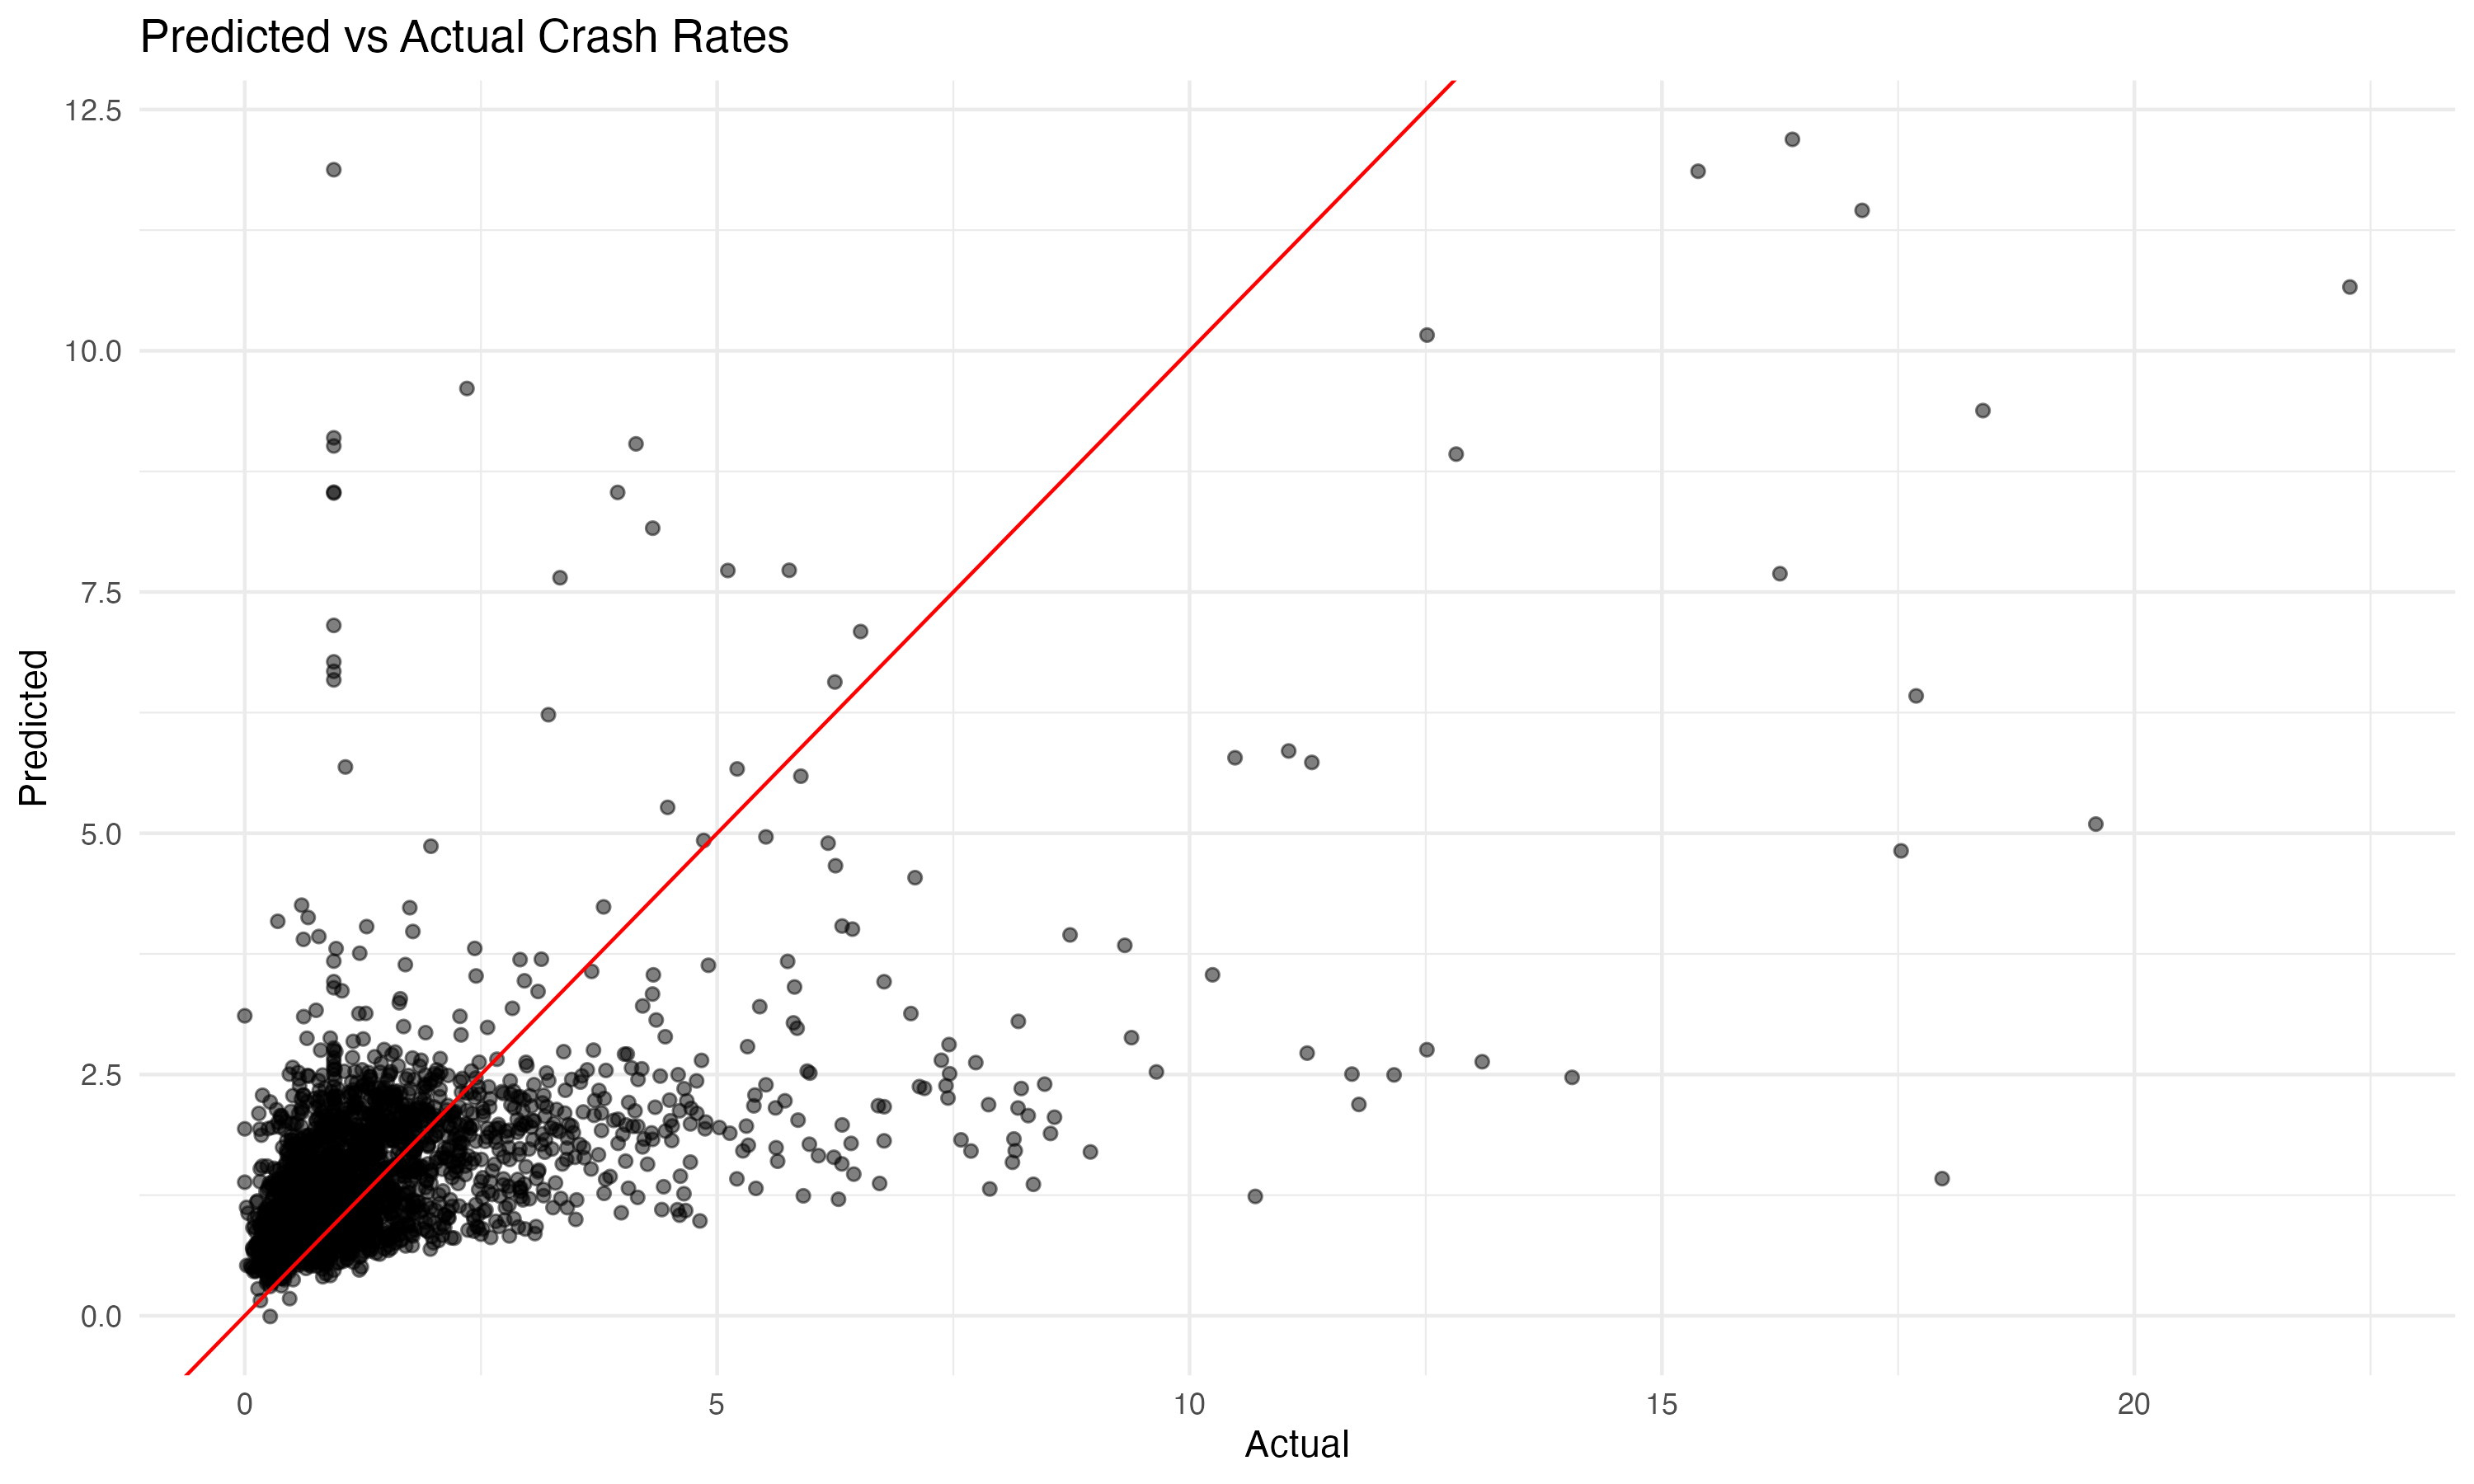
\includegraphics[keepaspectratio]{plots/predicted_vs_actual_values_plot.png}}

}

\caption{Predicted verses Actual Values on the Test Set}

\end{figure}%

The residual density plot indicates residuals are centered near zero
with a narrow peak, suggesting minimal systemic bias.

\begin{figure}[H]

{\centering \pandocbounded{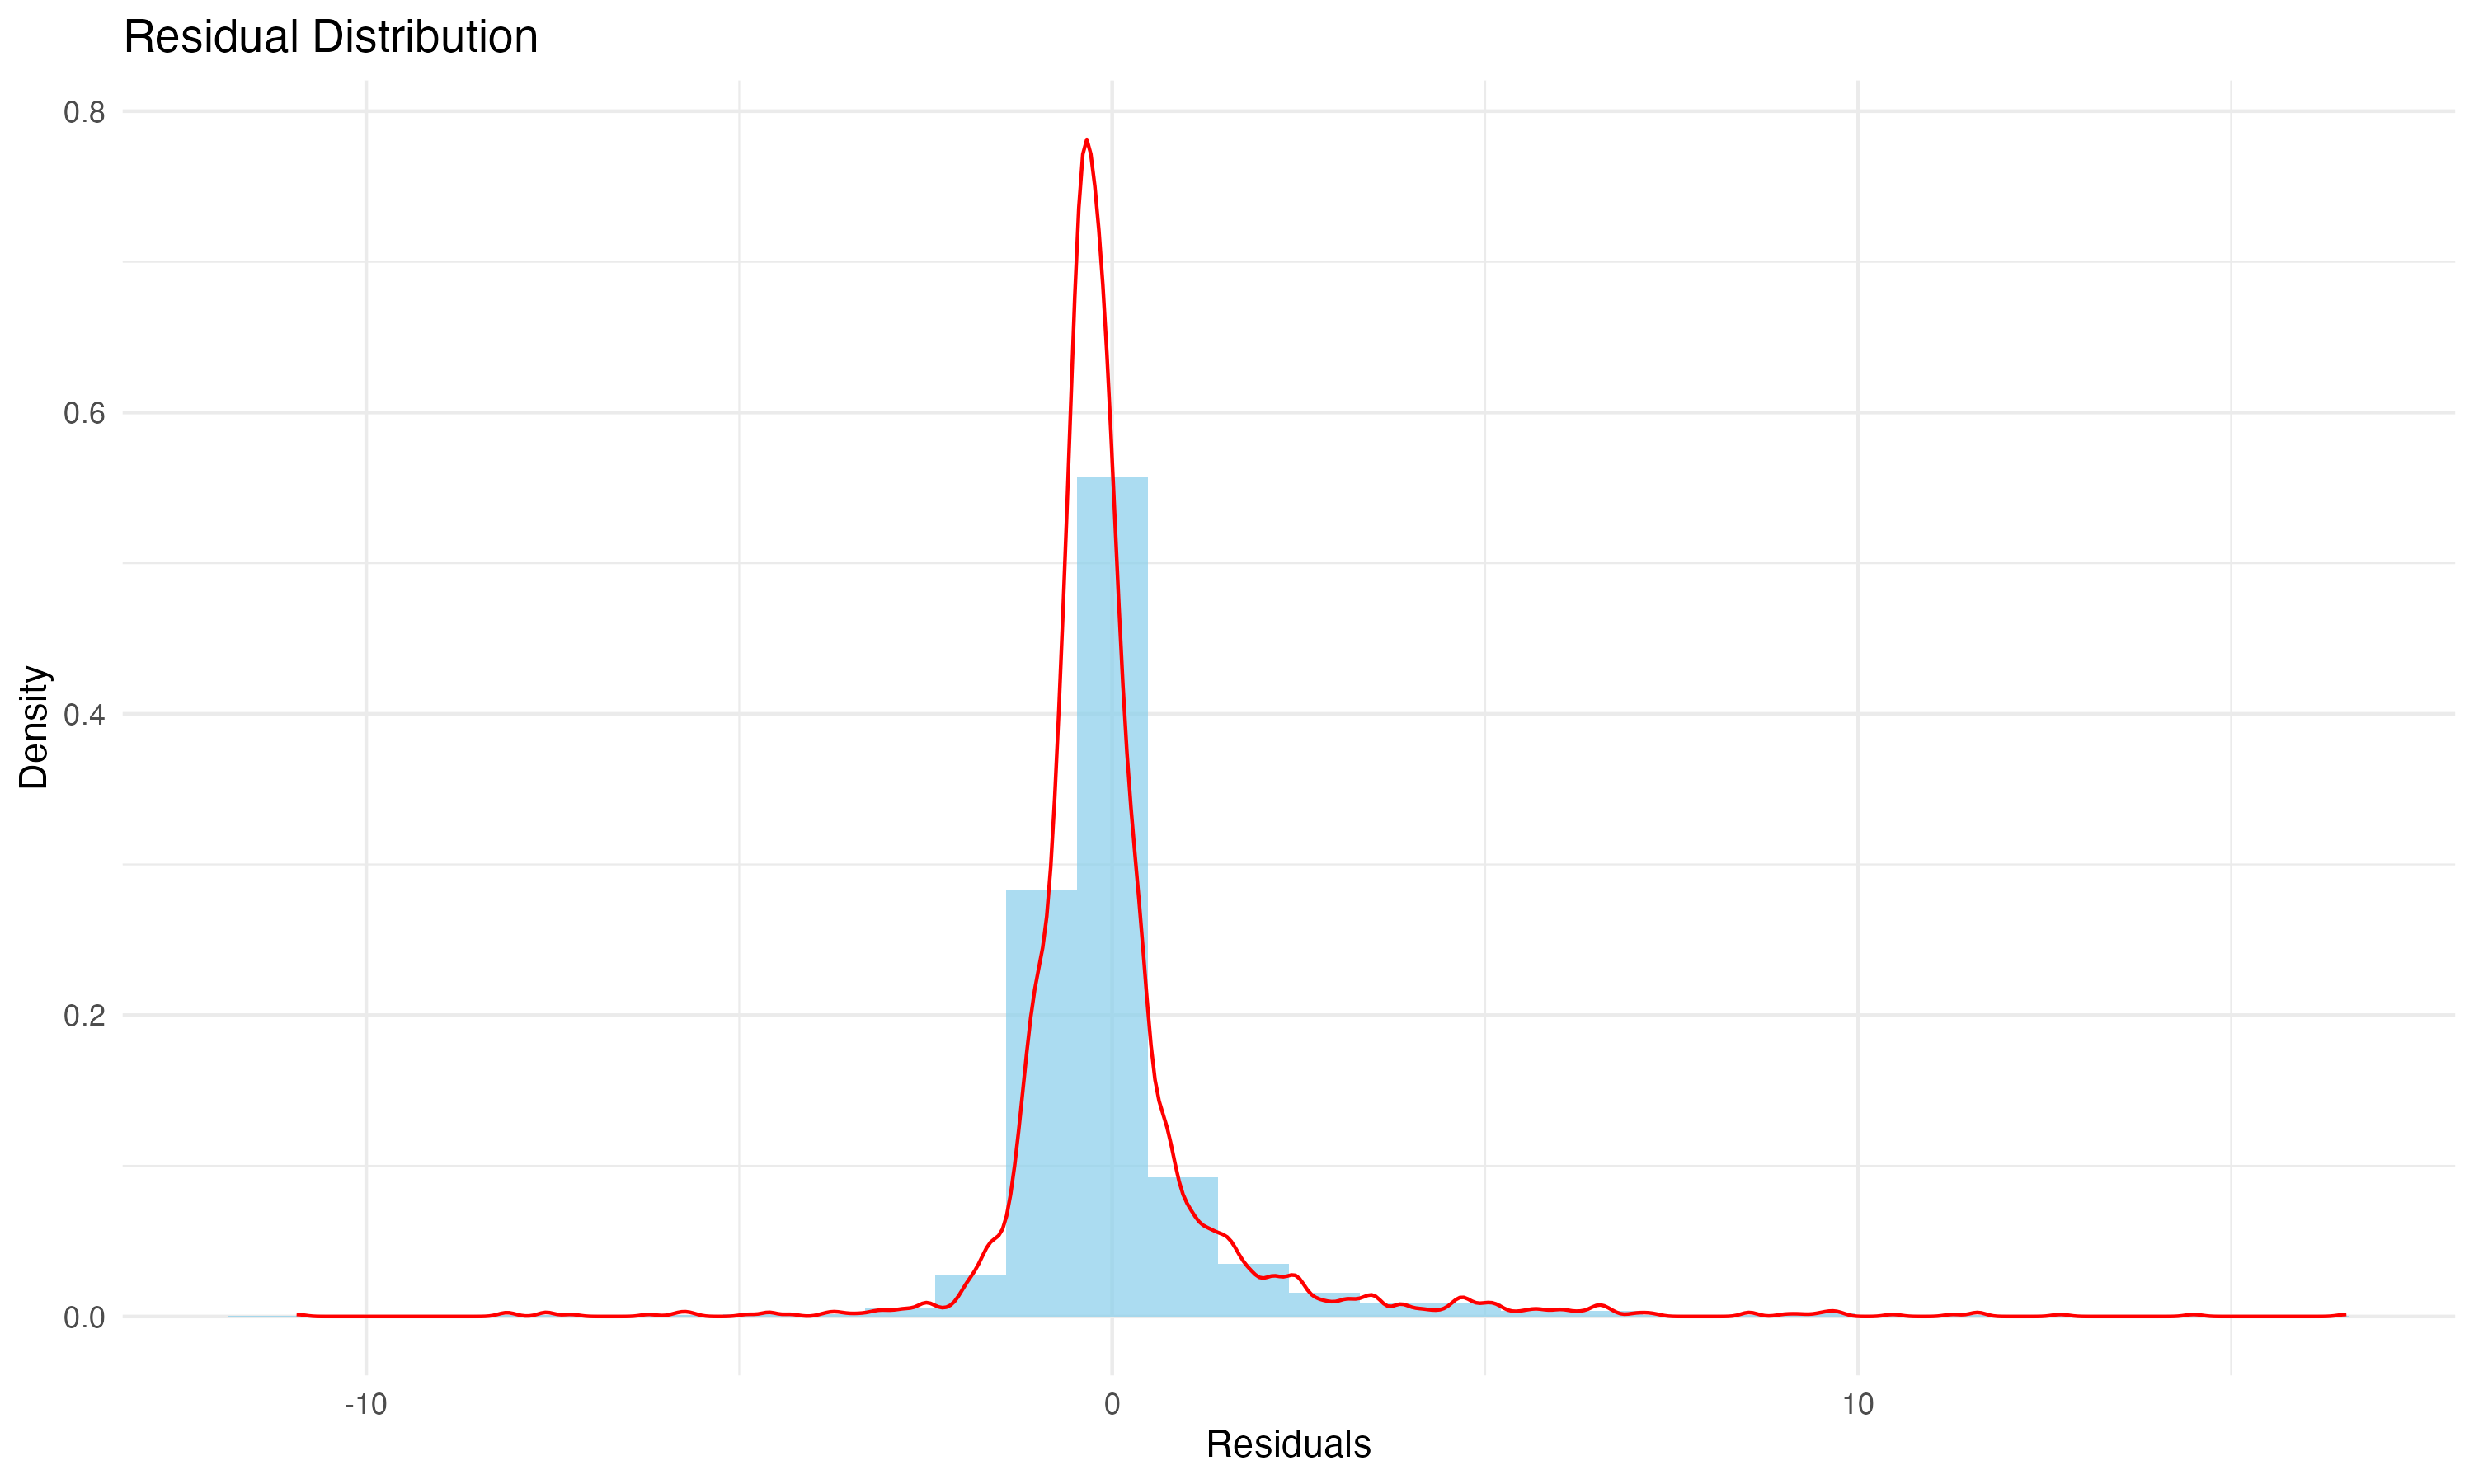
\includegraphics[keepaspectratio]{plots/residual_density_plot.png}}

}

\caption{Residual Density Plot}

\end{figure}%

The residuals vs.~predicted values plot shows a random scatter around
zero, with no strong patterns of heteroskedasticity or underfitting,
although a few outlier tracts exhibit residuals above ±10, likely due to
unique local conditions not captured by socio-economic predictors.

\begin{figure}[H]

{\centering \pandocbounded{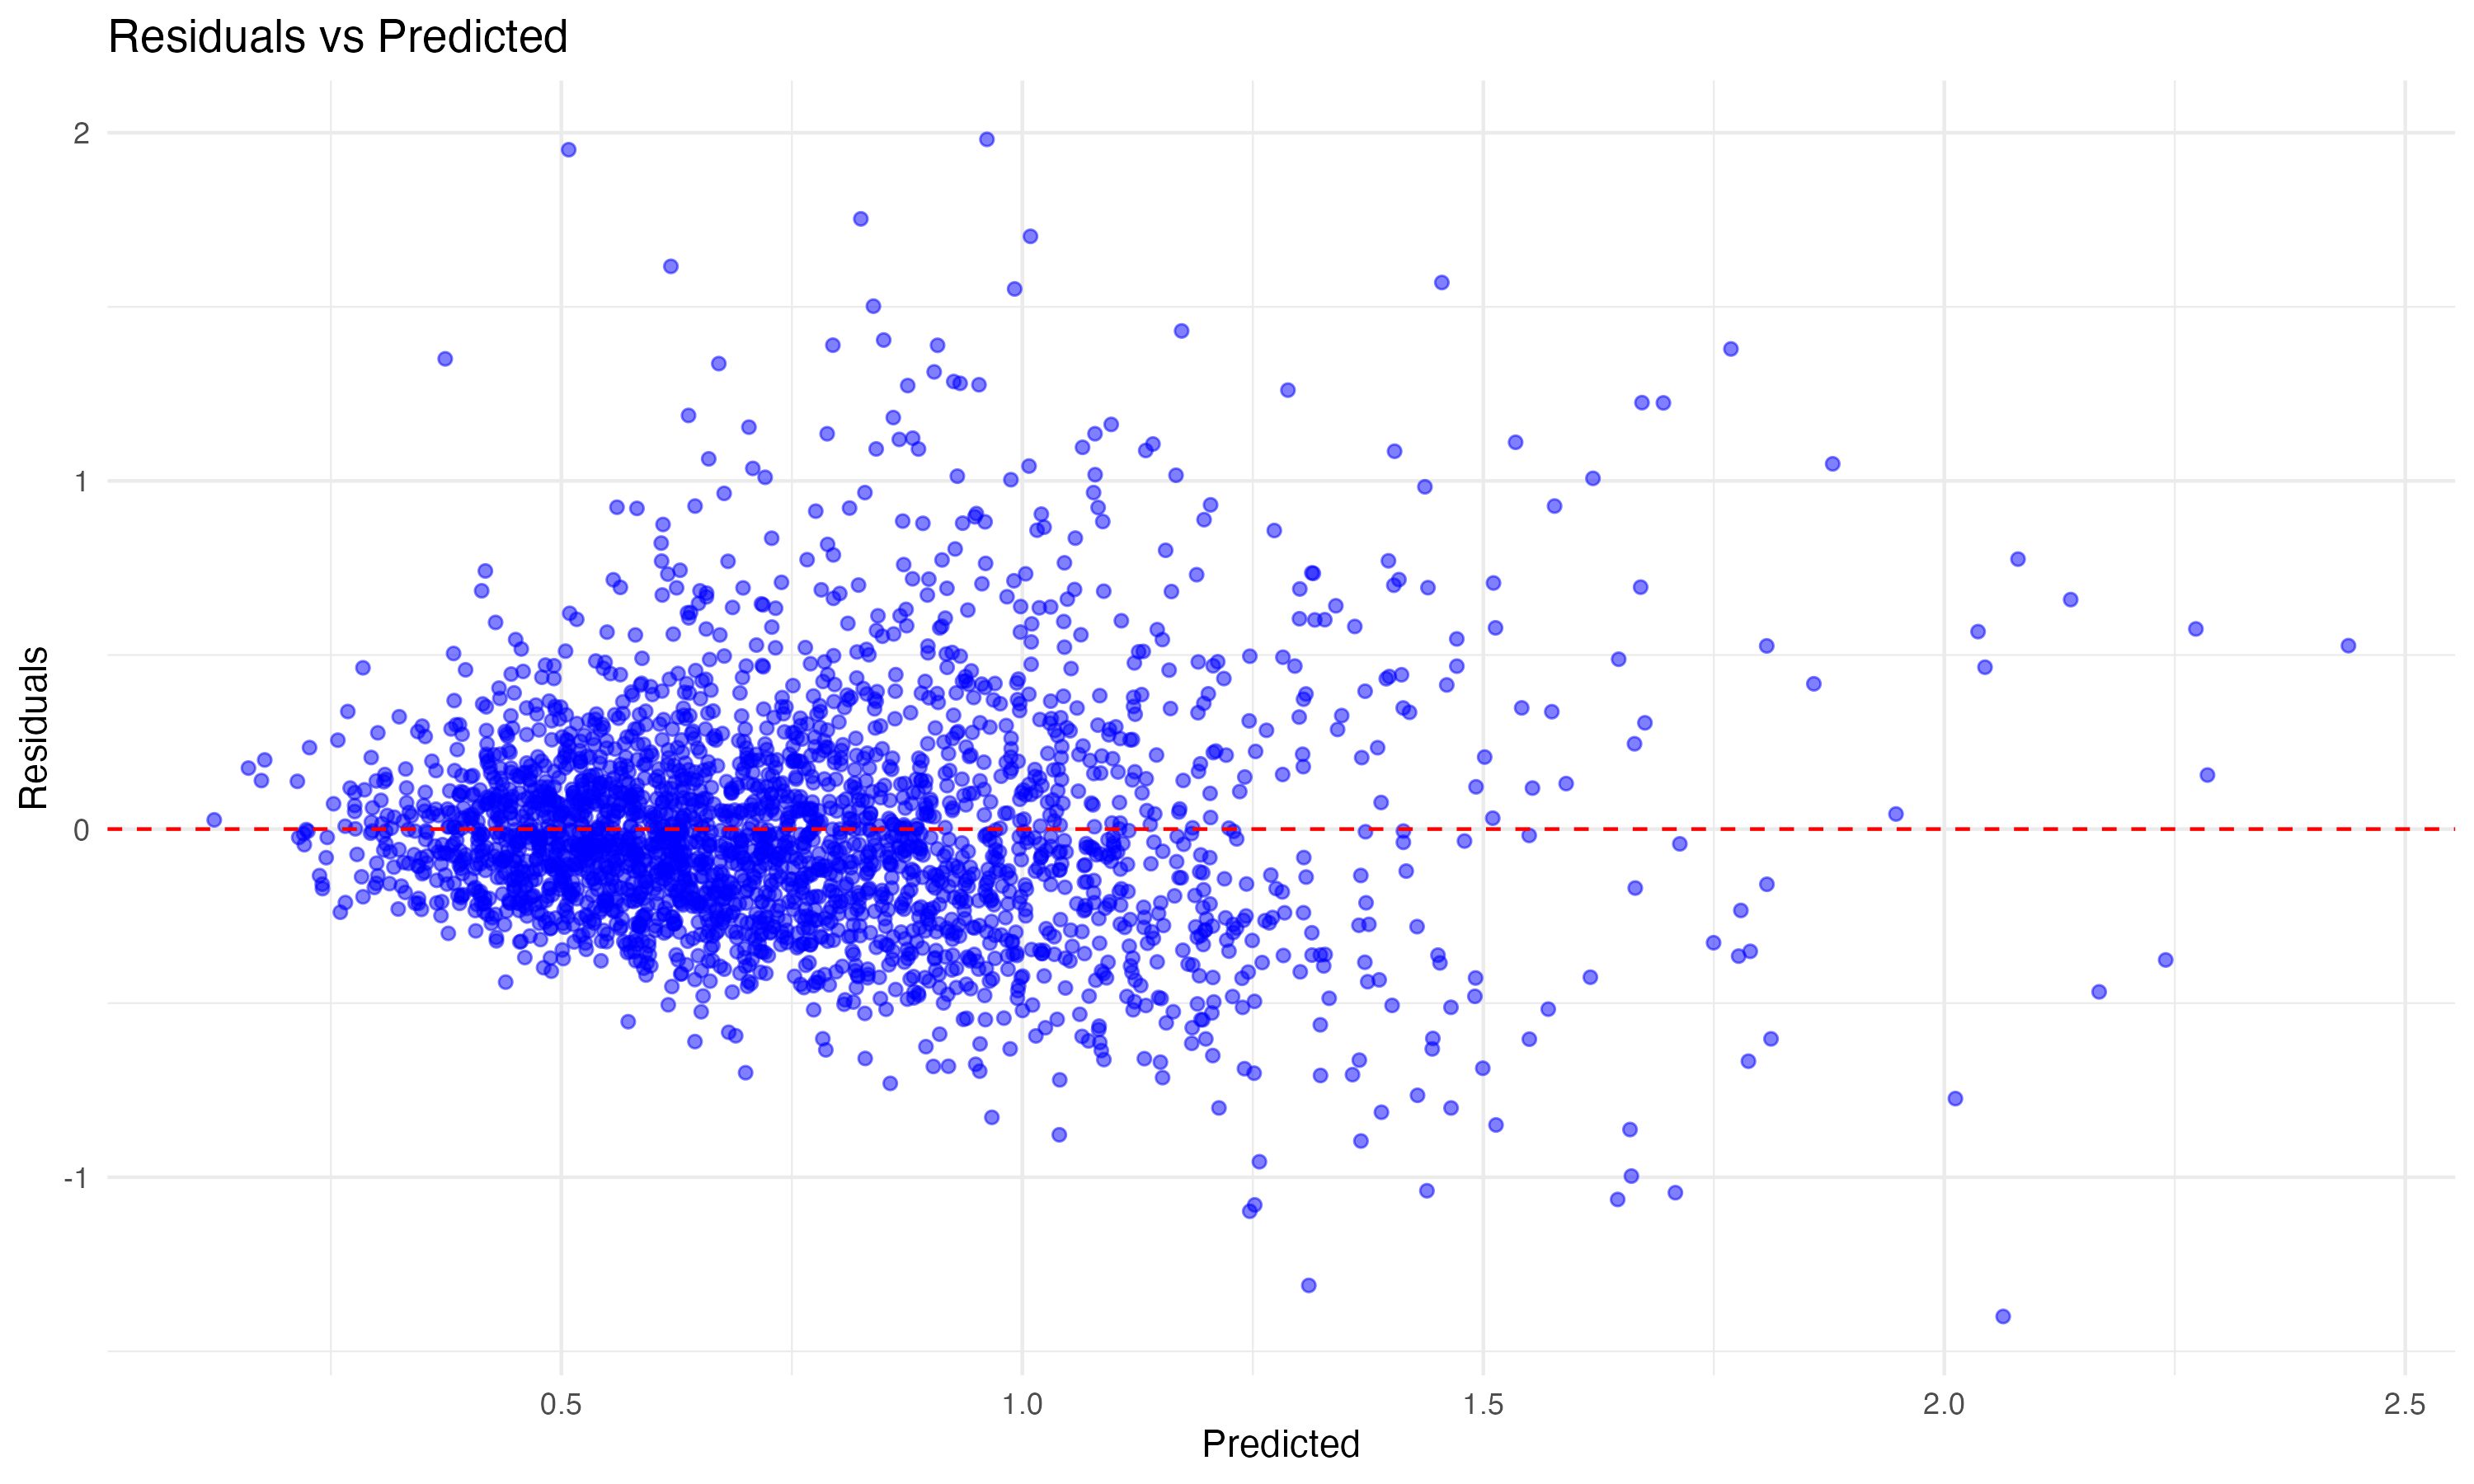
\includegraphics[keepaspectratio]{plots/resisuals_vs_predicted_values_plot.png}}

}

\caption{Residuals vs Predicted Values}

\end{figure}%

\begin{figure}[H]

{\centering \pandocbounded{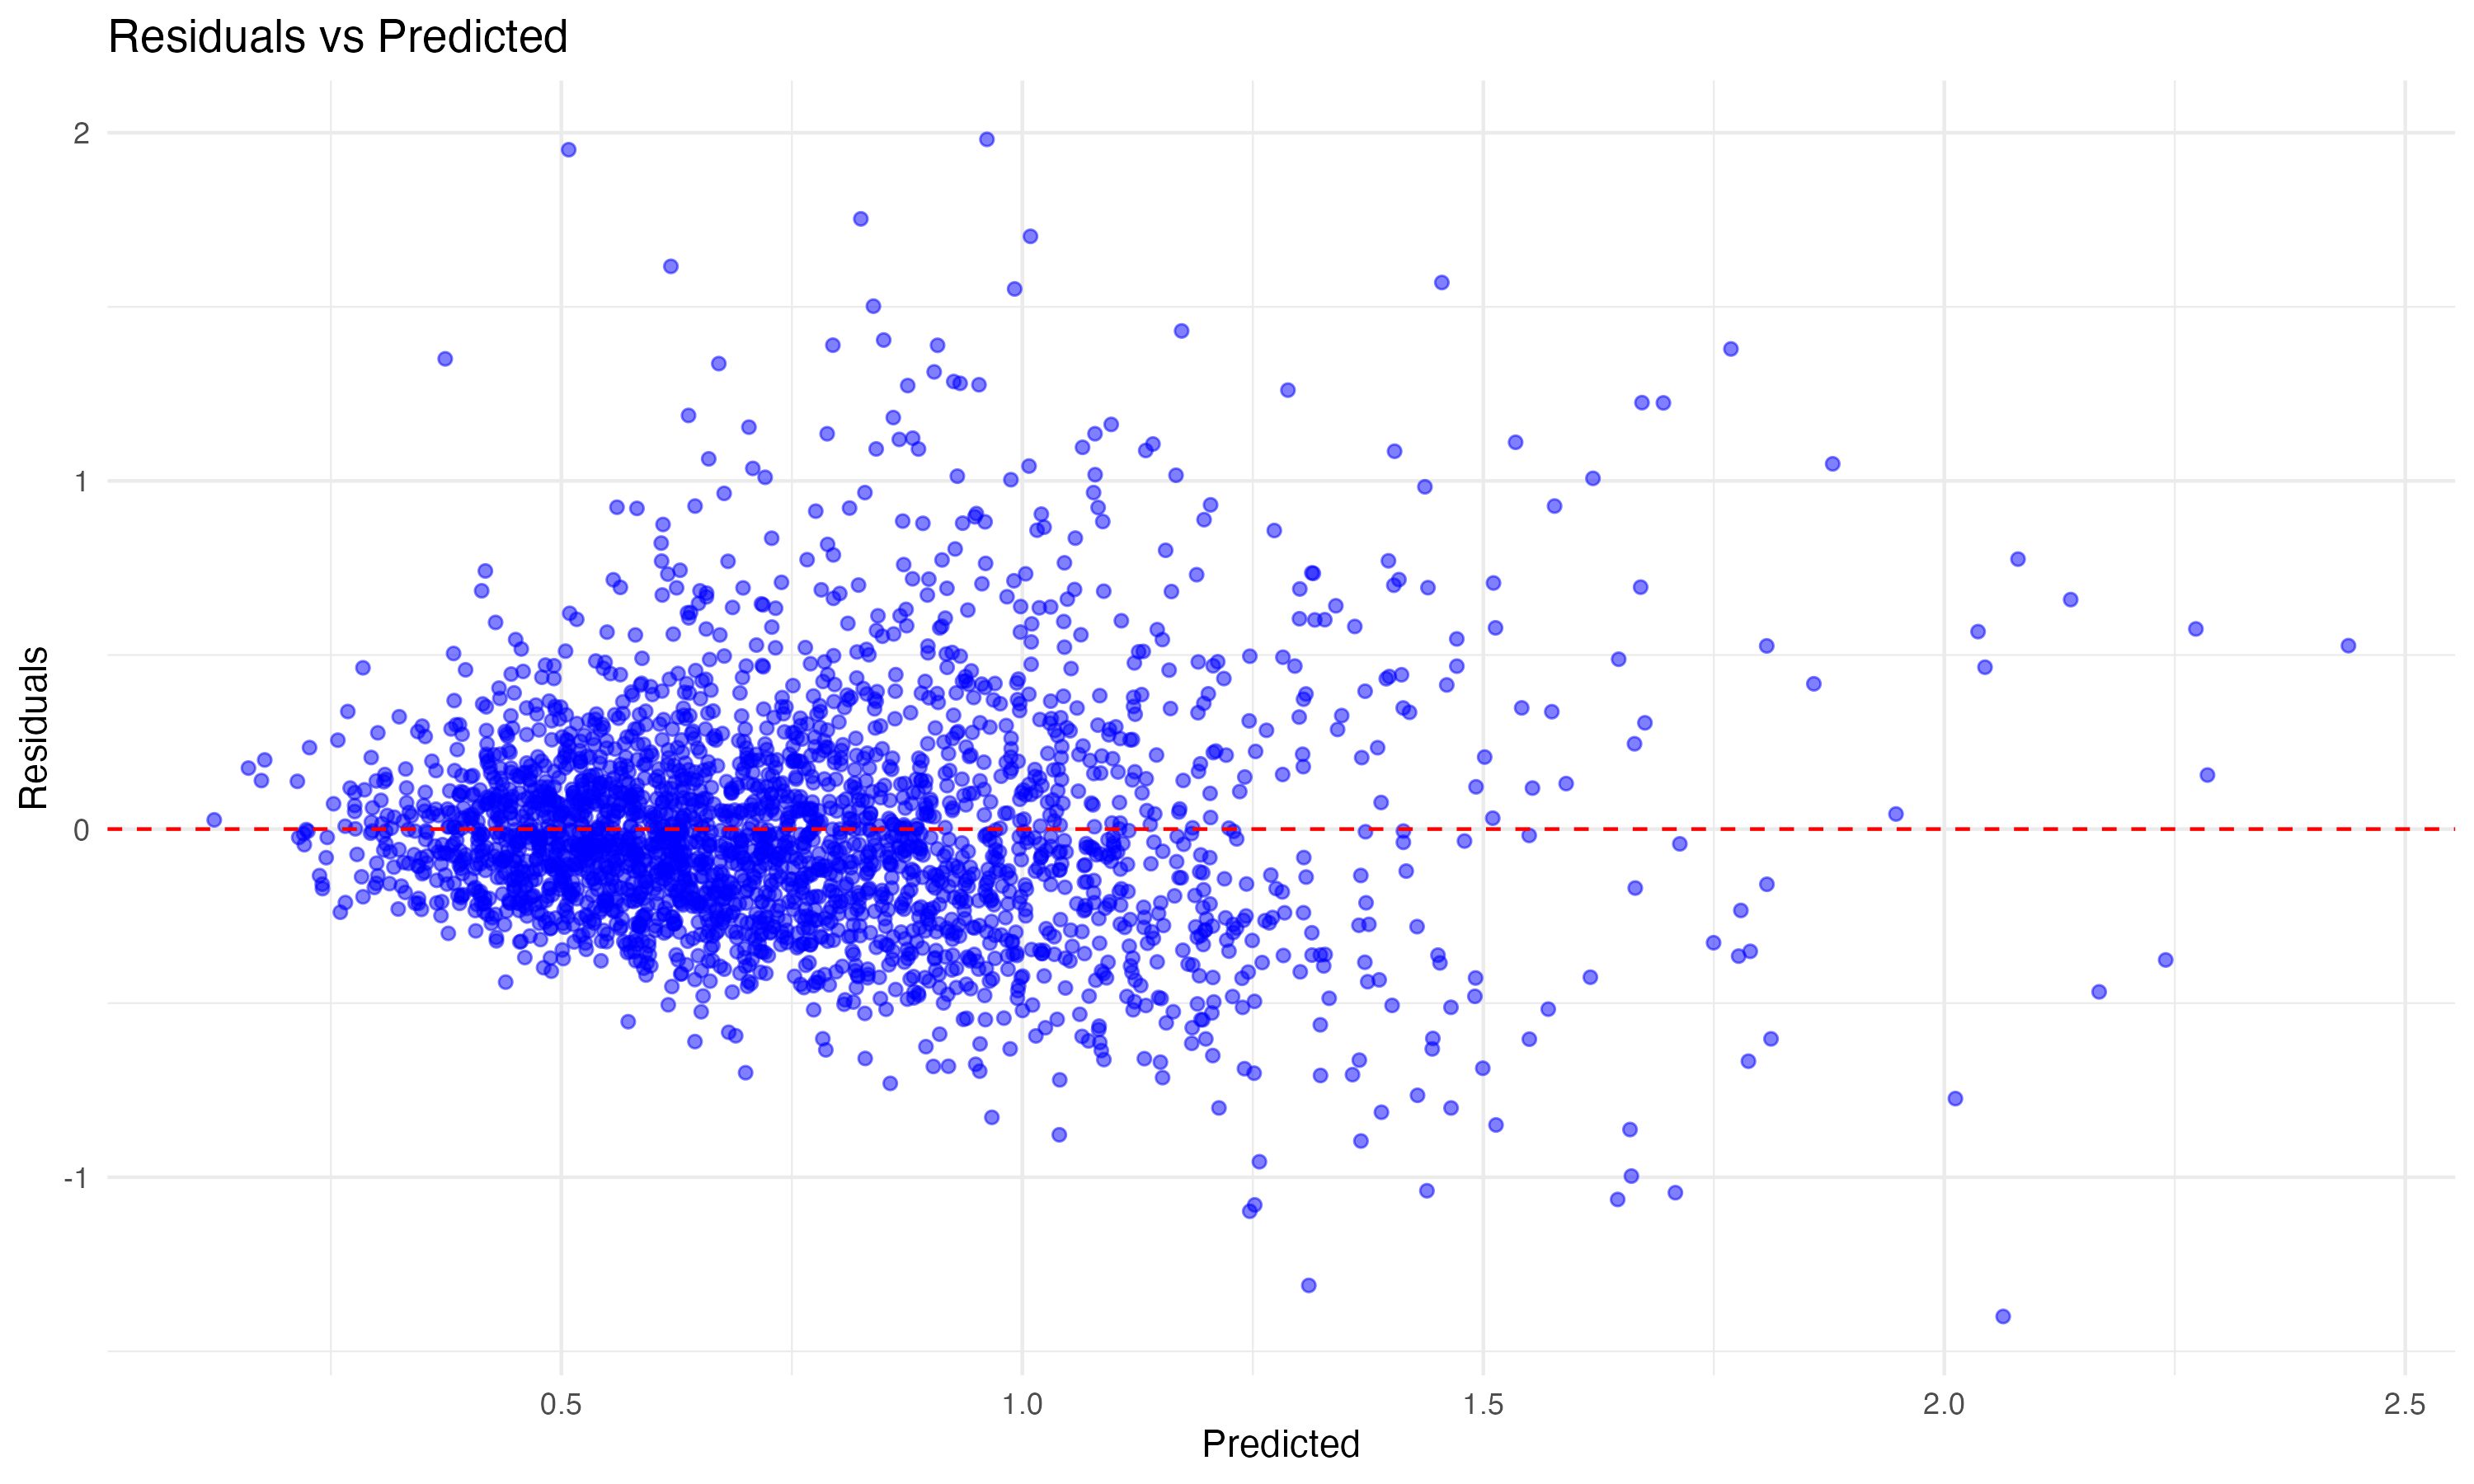
\includegraphics[keepaspectratio]{plots/resisuals_vs_predicted_values_plot.png}}

}

\caption{Global Feature Importance with SHAP}

\end{figure}%

\subsection{\texorpdfstring{\textbf{Global Feature Importance
(SHAP)}}{Global Feature Importance (SHAP)}}\label{global-feature-importance-shap}

The SHAP summary plot (Figure 5) highlights the most influential
features on crash risk predictions. The top 10 variables, in order of
importance, are:

\subsubsection{Post-Pandemic Indicator}\label{post-pandemic-indicator}

The post\_pandemic variableshows a marked upward shift in predicted
crash rates from 2020 onward, consistent with observed pandemic-era
changes in traffic dynamics (e.g., lower congestion but higher speeds).
This confirms that the temporal dimension significantly influences crash
risk beyond static socio-economic factors.

\subsubsection{Aging Population}\label{aging-population}

The PDP suggests that areas with a moderate share of elderly residents
(10--20\%) have slightly lower crash risks, potentially due to lower
driving exposure. However, beyond 20\%, predicted crash risk rises,
indicating that vulnerable road users like seniorsmay increase the
severity of crashes when incidents occur.

\subsubsection{High School Graduate
Population}\label{high-school-graduate-population}

For percent of the population with a high school diploma (but no further
education), the PDP exhibits a U-shaped relationship: tracts with either
very low or very high shares of residents holding a high school diploma
are associated with higher crash risk. This suggests that mid-level
education attainment may correlate with safer commuting patterns or less
risky behavior.

\subsubsection{Median Gross Rent}\label{median-gross-rent}

Median gross rent displays a positive gradient: tracts with higher
rents---often denser and more urbanized---show higher crash rates. This
likely reflects greater vehicle-pedestrian interactions and traffic
intensity in high-rent urban zones.

\subsubsection{Working Population}\label{working-population}

The PDP for percentage of the population in the workforce indicates that
crash risk peaks around 60--70\% labor force participation. Lower
participation areas may have fewer commuters, while areas with higher
participation rates may experience higher traffic volumes.

\subsubsection{Poverty Rate x Vehicle Ownership
Interaction}\label{poverty-rate-x-vehicle-ownership-interaction}

Th variable marking the interaction of vehicle ownership with poverty
rate shows that high poverty rates combined with high vehicle ownership
strongly elevate crash risk. This finding suggests that economically
vulnerable drivers may face both infrastructure and behavioral risks.

\begin{figure}[H]

{\centering \pandocbounded{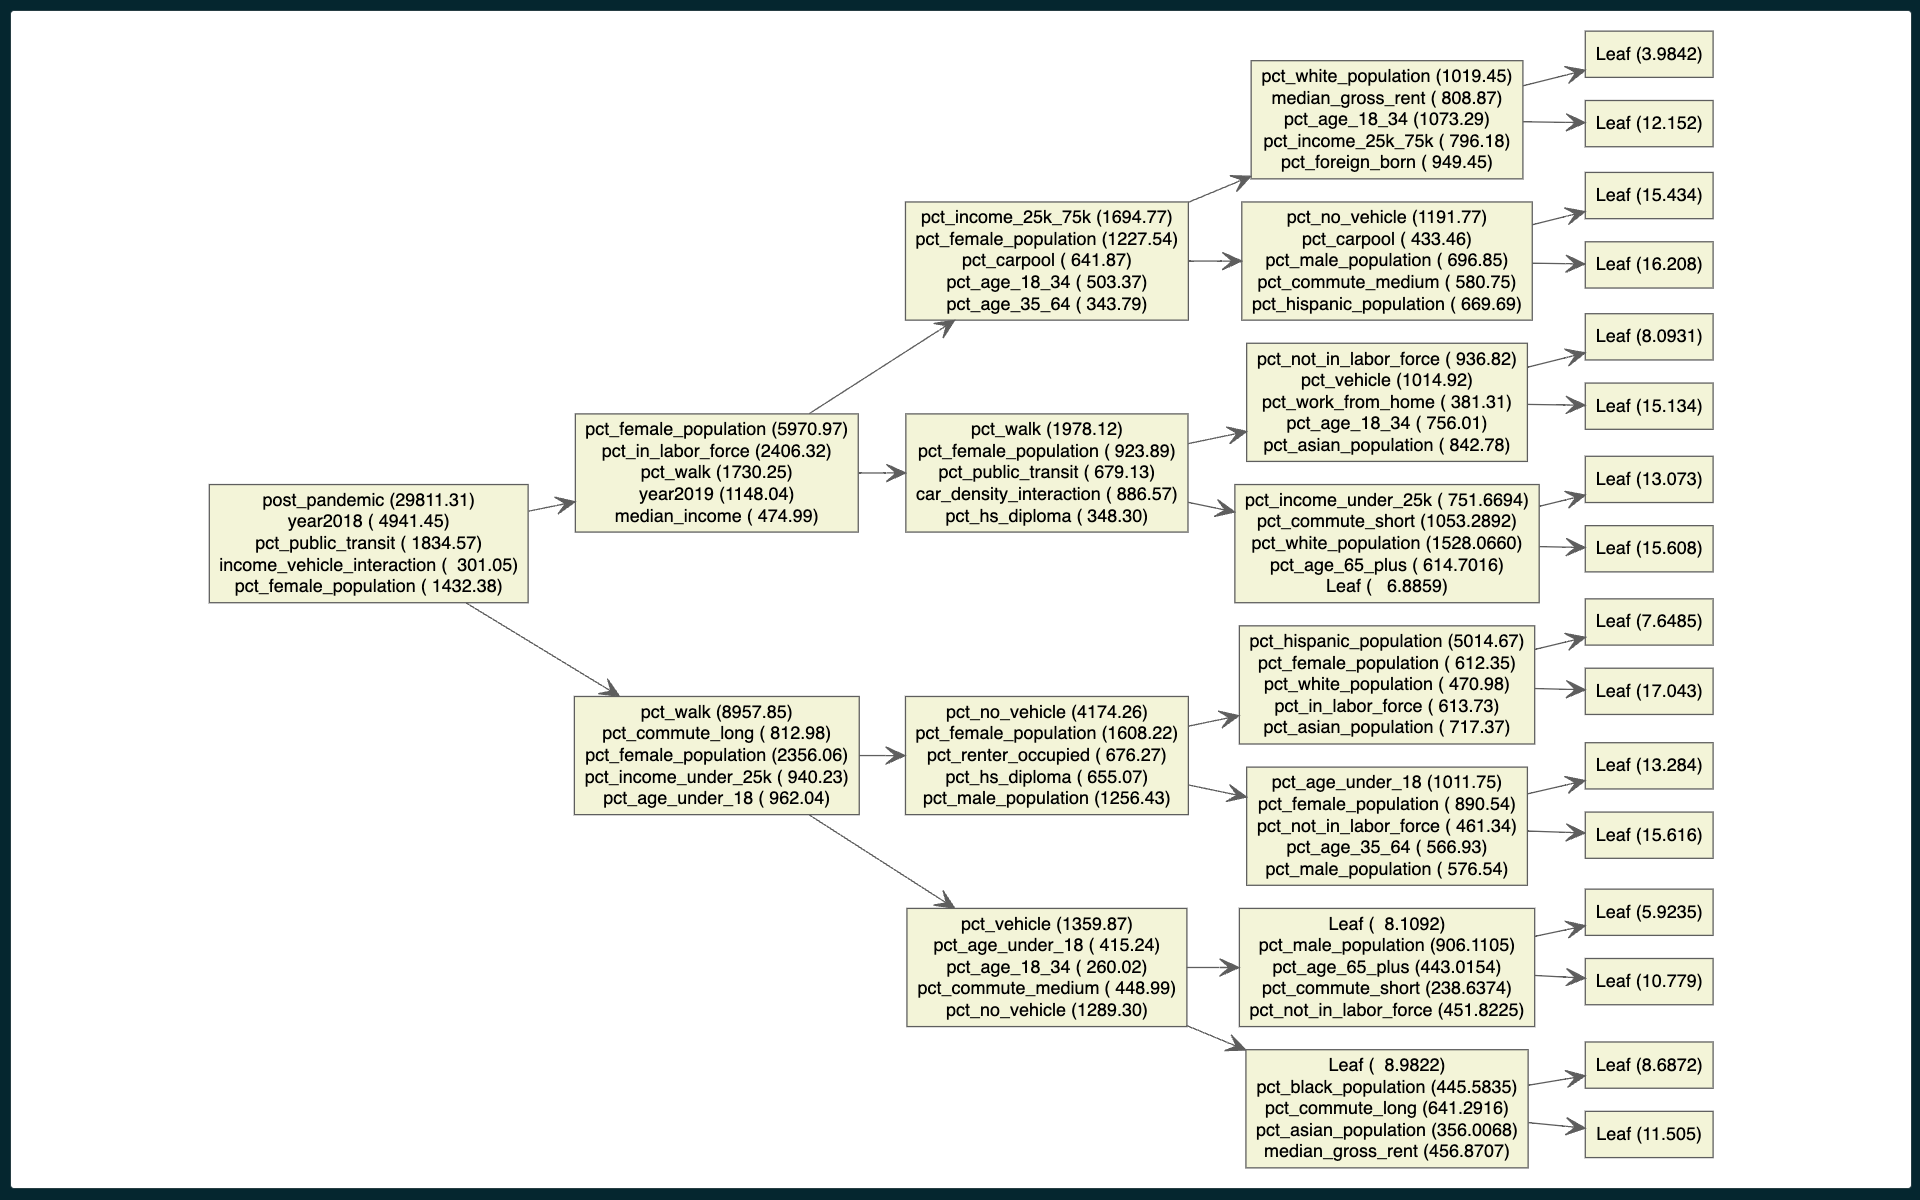
\includegraphics[keepaspectratio]{plots/multi_tree_plot.png}}

}

\caption{Figure X: Multi-Tree Plot}

\end{figure}%

\section{Discussion}\label{discussion}

The results of our gradient boosting model underscore both the potential
and the limitations of integrating socio-economic and transportation
indicators into auto insurance risk modeling. Although the model's R²
value of approximately 0.26 indicates that it explains just over
one-quarter of the variance in crash rates across New York City census
tracts, this is a meaningful achievement considering the inherent
randomness of crash events and the absence of individual-level data on
drivers and vehicles. Auto collisions are influenced by many unobserved
factors---such as momentary driver behavior, local weather conditions,
and road design---that cannot be captured through aggregated
socio-demographic measures alone. Despite these constraints, the model's
relatively low mean absolute error (0.84 crashes per 1,000 residents)
suggests that it has successfully captured consistent, broad patterns in
crash risk that align with socio-economic disparities and urban traffic
dynamics.

The SHAP analysis and multi-tree plot reveal that the most influential
predictors are not strictly transportation variables but rather
socio-economic indicators that shape exposure and vulnerability. The
post-pandemic indicator emerges as the single strongest factor,
reflecting the profound shift in traffic patterns since 2020, when less
congestion but higher average speeds increased crash severity. This
temporal variable, acting as a structural change marker, underscores how
risk is not static and can be dramatically influenced by societal
events. Other dominant features include the percentage of the population
aged 65 and older, which is associated with heightened crash severity
likely due to the increased vulnerability of older pedestrians and
drivers. The model suggests a non-linear relationship: neighborhoods
with a moderate share of elderly residents (10--20\%) have slightly
lower risk---perhaps due to reduced driving exposure---while higher
concentrations of elderly populations increase risk due to physical
fragility and slower response times during collisions.

Housing and economic variables also feature prominently. Median gross
rent is positively correlated with crash rates, suggesting that denser,
higher-cost urban areas, with more vehicle-pedestrian interactions and
complex traffic flows, have elevated risk levels. Similarly, labor force
participation peaks as a predictor around 60--70\%, reflecting that
areas with higher commuter activity experience more traffic and thus
more collisions. The inclusion of income distribution
metrics---particularly the share of households earning under \$25,000
and between \$25,000--\$75,000---highlights how economic vulnerability
and mid-range income commuting patterns interact to shape risk exposure.

One of the most striking findings is the role of poverty × vehicle
ownership interaction, which appears consistently in the multi-tree
plot. Areas with both high poverty rates and high vehicle availability
show notably higher crash risks, likely due to a combination of older
vehicles, reduced access to safety infrastructure, and potentially
riskier driving environments. This aligns with prior research linking
socio-economic deprivation to both higher accident rates and more severe
outcomes due to disparities in road safety infrastructure and
enforcement intensity.

From a social risk modeling perspective, these results are significant.
The SHAP-derived importance of variables like percent of the population
walking or biking, public transit use, and commute time reflects how
transportation mode choice is strongly tied to risk exposure. For
example, tracts with higher walking or biking shares---especially when
combined with high rents or dense populations---are more likely to see
pedestrian or cyclist-involved accidents. Similarly, higher public
transit usage can act as both a risk mitigator (reducing car volume) and
a risk amplifier in areas with heavy pedestrian traffic near transit
hubs.

While the model demonstrates that neighborhood-level demographic and
economic factors can act as strong proxies for crash risk, it also
highlights critical limitations for deployment in insurance pricing. The
moderate R² indicates that a significant portion of risk remains
unaccounted for, largely due to unobserved individual-level factors such
as driver age, prior claims, and vehicle safety features. Moreover, the
use of variables like income, race, or foreign-born population---though
statistically predictive---would be highly problematic if directly
incorporated into premium calculations due to both legal prohibitions
(e.g., anti-discrimination laws) and ethical concerns. These variables
risk proxy discrimination, where protected classes are indirectly
penalized through correlated socio-economic attributes.

The model answers our primary research question---whether publicly
available socio-economic and crash data can be combined to model
geographic risk---and the answer is a qualified yes. It shows that these
factors can explain spatial patterns of crashes and provide insurers or
policymakers with macro-level risk insights. However, the model cannot,
and should not, be used as-is for individual risk assessment. It is
better suited for regional portfolio analysis, identifying high-risk
neighborhoods for targeted safety interventions, or supplementing
traditional actuarial models rather than replacing them.

Moving forward, future research should focus on enhancing the model's
granularity and fairness. Incorporating telematics data, which captures
real-time driving behavior (speeding, braking, distance driven), could
greatly increase predictive accuracy while avoiding over-reliance on
socio-economic proxies. Similarly, integrating temporal modeling
techniques---such as time-series gradient boosting or hybrid approaches
with recurrent neural networks---would enable the model to capture
seasonal and event-driven variations in crash risk. Additionally,
fairness-aware machine learning techniques could be applied to mitigate
the risk of socio-economic bias while maintaining predictive
performance.

\section{Conclusions and Future Work}\label{conclusions-and-future-work}

This research demonstrates that gradient boosting, combined with
socio-economic and crash data, can provide interpretable, data-driven
insights into auto insurance risk patterns in NYC. By identifying key
drivers of crash risk---such as post-pandemic shifts, commuting
intensity, and socio-economic vulnerability---the model offers a
foundation for both urban safety planning and high-level risk
assessment.

Yet, the study's findings also underscore the limitations of using
aggregated, public data for underwriting. While the model captures broad
trends, it lacks the precision, granularity, and fairness safeguards
required for production-level insurance applications. Therefore, the
model is best suited as a complementary tool for insurers, providing
neighborhood-level risk insights or supporting reinsurance and portfolio
management rather than individual pricing.

Future research should focus on three fronts: (1) integrating behavioral
data, such as telematics, to bridge the gap between macro-level
socio-economic patterns and micro-level driving behavior; (2) developing
fairness-aware modeling approaches to mitigate bias from socio-economic
proxies; and (3) exploring temporal extensions that incorporate evolving
risk factors, including post-pandemic traffic patterns and
climate-related hazards. These directions will help transition from
descriptive social risk modeling to actionable, ethically sound
insurance applications.

\section{Appendix A: Variables
Modeled}\label{appendix-a-variables-modeled}

\begin{longtable}[]{@{}
  >{\raggedright\arraybackslash}p{(\linewidth - 6\tabcolsep) * \real{0.1210}}
  >{\raggedright\arraybackslash}p{(\linewidth - 6\tabcolsep) * \real{0.2984}}
  >{\raggedright\arraybackslash}p{(\linewidth - 6\tabcolsep) * \real{0.4516}}
  >{\raggedright\arraybackslash}p{(\linewidth - 6\tabcolsep) * \real{0.1290}}@{}}
\caption{Table 2: Key variables, descriptions, and transformations in
the final dataset.}\tabularnewline
\toprule\noalign{}
\begin{minipage}[b]{\linewidth}\raggedright
Variable
\end{minipage} & \begin{minipage}[b]{\linewidth}\raggedright
Description
\end{minipage} & \begin{minipage}[b]{\linewidth}\raggedright
Type
\end{minipage} & \begin{minipage}[b]{\linewidth}\raggedright
Transformation
\end{minipage} \\
\midrule\noalign{}
\endfirsthead
\toprule\noalign{}
\begin{minipage}[b]{\linewidth}\raggedright
Variable
\end{minipage} & \begin{minipage}[b]{\linewidth}\raggedright
Description
\end{minipage} & \begin{minipage}[b]{\linewidth}\raggedright
Type
\end{minipage} & \begin{minipage}[b]{\linewidth}\raggedright
Transformation
\end{minipage} \\
\midrule\noalign{}
\endhead
\bottomrule\noalign{}
\endlastfoot
Demographic & pct\_male\_population & Men & Percentage \\
Demographic & pct\_white\_population & Identifying as white &
Percentage \\
Demographic & pct\_black\_population & Identifying as black &
Percentage \\
Demographic & pct\_asian\_population & Identifying as Asian &
Percentage \\
Demographic & pct\_hispanic\_population & Identifying as Hispanic/Latino
& Percentage \\
Demographic & pct\_foreign\_born & Foreign-born & Percentage \\
Age & pct\_age\_under\_18 & Under 18 & Percentage \\
Age & pct\_age\_18\_34 & Aged 18-34 & Percentage \\
Age & pct\_age\_35\_64 & Aged 35-64 & Percentage \\
Age & pct\_age\_65\_plus & Aged 65 and above & Percentage \\
Income/Poverty & median\_income & Median household income
(inflation-adjusted) & Raw value (USD) \\
Income/Poverty & pct\_income\_under\_25k & Households earning less than
\$25,000 & Percentage \\
Income/Poverty & pct\_income\_25k\_75k & Households earning
\$25,000-\$75,000 & Percentage \\
Income/Poverty & pct\_below\_poverty & Below the poverty line &
Percentage \\
Housing & median\_gross\_rent & Median gross rent (USD) & Raw value
(USD) \\
Housing & pct\_owner\_occupied & Owner-occupied housing units &
Percentage \\
Housing & pct\_renter\_occupied & Renter-occupied housing units &
Percentage \\
Education & pct\_less\_than\_hs & Less than high school education &
Percentage \\
Education & pct\_hs\_diploma & High school diploma & Percentage \\
Education & pct\_some\_college & Some college education & Percentage \\
Education & pct\_associates\_degree & Associate's degree & Percentage \\
Education & pct\_bachelors\_degree & Bachelor's degree & Percentage \\
Education & pct\_graduate\_degree & Graduate or professional degree &
Percentage \\
Employment & pct\_in\_labor\_force & In the labor force & Percentage \\
Employment & unemployment\_rate & Unemployment rate & Percentage \\
Transport & pct\_commute\_short & Commute under 15 minutes &
Percentage \\
Transport & pct\_commute\_medium & Commute between 15-30 minutes &
Percentage \\
Transport & pct\_commute\_long & Commute longer than 30 minutes &
Percentage \\
Transport & pct\_carpool & By carpool & Percentage \\
Transport & pct\_public\_transit & By public transit & Percentage \\
Transport & pct\_walk & By walking & Percentage \\
Transport & pct\_bike & By biking & Percentage \\
Transport & pct\_work\_from\_home & Working from home & Percentage \\
Transport & pct\_vehicle & Owns a vehicle & Percentage \\
Engineered & post\_pandemic & Post-pandemic indicator (1 = 2020 and
later) & Binary \\
Engineered & poverty\_vehicle & & \\
\_interaction & Interaction term: poverty rate × vehicle ownership &
Interaction & \\
Engineered & unemployment\_vehicle & & \\
\_interaction & Interaction term: unemployment rate × vehicle ownership
& Interaction & \\
Year & year2018 & Year dummy: 2018 & Indicator \\
Year & year2019 & Year dummy: 2019 & Indicator \\
Year & year2020 & Year dummy: 2020 & Indicator \\
Year & year2021 & Year dummy: 2021 & Indicator \\
Year & year2022 & Year dummy: 2022 & Indicator \\
Year & year2023 & Year dummy: 2023 & Indicator \\
\end{longtable}


\renewcommand\refname{References}
\bibliography{bibliography.bib}



\end{document}
